\chapter{Introduction}
\label{chapter-introduction}

Embedded systems present difficult programming challenges
\cite{Mottola:2011:PWS:1922649.1922656}. For reasons of size, power consumption, disposability,
or some combination of these things, embedded devices are often highly resource constrained. For
example, a typical device might have only 48\,KiB of program ROM, 10\,KiB of RAM, and use a
small, 16~bit microcontroller running at 8\,MHz \cite{tmotesky-datasheet}. Yet embedded
applications are increasing in complexity and often provide mission-critical or even
safety-critical services. Such systems need to be both efficient and correct.

This dissertation specifically looks at the problem of providing distributed trust management in
resource constrained embedded systems. Here \newterm{trust management} refers to a general
approach for authorizing access to resources in an environment where the identity of requesting
principals is not known to the authorizer. A trust management system provides a way for the
authorizer to define an access policy in terms of arbitrary certified attributes that the
requester must possess. Many trust management systems have been described in the literature
\cite{chapin-skalka-wang-acmcs08}, and they vary in complexity, expressivity, and mathematical
foundations. However, they all attempt to provide a well structured approach to the problem of
access control in widely distributed and dynamic environments.

Trust management systems are typically designed for use by authorizers with resource rich
machines such as is commonly used for file and web servers. To the knowledge of this author,
trust management has never before been demonstrated in a deeply embedded context. Yet there are
embedded applications that could also benefit from trust management. For example, ``smart cars''
that communicate with each other about road conditions \cite{Seepold:2009:ESP:1641563.1641568},
or body area networks that provide medical monitoring features
\cite{Shnayder:2005:SNM:1098918.1098979,Chen:2011:BAN:1968858.1968873}, may encounter many
unknown principals during their operation. The security and safety of these applications, and
many others, will depend on their ability to distinguish trustworthy principals from unreliable
or malicious ones.

For reasons of space and time efficiency, many embedded systems are programmed in low level
languages such as C. Programming at that level is complicated and error prone. It is desirable,
therefore, to provide programmers with convenient abstractions to shield them from low level
complexities. These abstractions should be in the programming language itself, and this
dissertation is about providing enriched languages that can address the needs of modern embedded
systems in general and the embedded trust management problem in particular. This
\newterm{language-based} approach moves some of the work of producing correct programs to the
language compiler and runtime system. Language features can be formally analyzed and rigorously
tested once and then applied to many applications. This is in contrast to each application being
an ad-hoc construction of customized components with limited use beyond the application for
which they were created.

The value of formal foundations cannot be overstated. In critical systems where safety or
security is at stake, a rigorous understanding of the mechanisms being used is essential. For
example, trust management systems that provide a precisely defined policy language are
preferable to systems that use informal methods.

The focus of this dissertation is on a kind of embedded system called a \newterm{wireless sensor
  network} (WSN). Such systems consist of a network of small sensors or actuators that are
connected by way of short hop wireless links. Commonly such networks include one or more base
stations, or ``hubs,'' with wider connectivity that serve as an interface between the sensor
network and external systems. Wireless sensor networks are an area of intense study with many
envisioned applications ranging from environment, asset, and structural monitoring to emergency
response \cite{Culler:2004:GEI:1018015.1018072,1038146}. Yet despite the use of sensor networks
to demonstrate the systems described herein, the techniques can be used with a wide range of
embedded applications.

Two approaches to solving the problem of providing trust management-style distributed
authorization in resource constrained embedded systems are discussed here. The first approach is
based on a new remote procedure call (RPC) discipline named \textit{SpartanRPC}
\cite{chapin-skalka-SpartanRPC,chapin-skalka-SpartanRPCTR}. In this method all trust management
computations are done directly on the embedded devices. However, the complexity of the system is
hidden from the programmer behind a simple extension to the widely used nesC programming
language \cite{Gay-nesC-2003}. In order to implement this \emph{direct} approach, a compiler
called \textit{Sprocket}, that takes an extended dialect of the nesC language as input and
outputs an equivalent program in ordinary nesC, has been created. In addition Sprocket outputs
the necessary runtime support to process authorization requests and policy statements in the
$RT_0$ trust management language \cite{Li:DRBTMF,Li:RRBTMF}.

The second approach presented is based on \newterm{staged programming}
\cite{Taha-MetaML,Sheard-TemplateHaskell,Mainland-Flask-2008,FramedML}. In a staged environment,
a first stage program is used to compose and specialize a lower level, second stage, program.
Specialized code can often be considerably optimized. However, flexibility is retained because
the first stage program can be re-executed at a later time to re-specialize the second stage
program as needed.

Unlike with many staging systems, the work described here uses stages with different programming
languages and that execute on different machines, i.e., in different address spaces. When
applied to embedded systems the second (and final) stage must be in an embedded systems language
running on the embedded hardware, whereas the first stage need not be as restricted.

This dissertation also describes \newterm{Scalaness} \cite{chapin-GPCE-2013}, an extension of
Scala \cite{PiS2} with features that allow the programmer to compose and specialize components
written in a reduced dialect of nesC, which is called \newterm{nesT}. An important and novel
feature of Scalaness is that it extends Scala's type system, so that a well-typed Scalaness
program will always generate a well-typed nesT program. Thus, the type correctness of the
program that ultimately runs on the embedded device is guaranteed by the first stage Scalaness
compiler.

Scala was chosen as the basis for the first stage language largely for pragmatic reasons,
primarily to build a system that could be used for real applications. Scala is a rich language
that runs on the Java Virtual Machine (JVM) and has access to the Java ecosystem. Also the Scala
compiler has a plugin architecture, and it was originally intended to implement Scalaness as a
compiler plugin. Unfortunately, as described in \autoref{chapter-scalaness-nest} that proved
difficult and Scalaness was instead implemented as a direct modification to the Scala compiler
itself.

\section{Motivation}

%%%%%
% Start of first responder application. Where to put it?
%%%%%

As an example of an application that illustrates the concepts of trust management in embedded
systems, consider a first responder situation in which multiple social entities must interact
and cooperate. Recent work has shown the effectiveness of wireless sensor networks in such
scenarios \cite{citeulike:4460555,1038146} in their ability to coordinate multiple data
collection and communication devices in an ad-hoc, easily deployable fashion. However, data
collection and communication in this scenario (and other similar ones) must be a secured
resource, due to, e.g., HIPA requirements in the case of medical response. Furthermore, security
must be coordinated on-site in a sensor network comprising subnetworks administered separately
(police, medical units from different hospitals, etc.), and no prior coordination between
administrations can generally be assumed. Trust management authorization is well suited for this
kind of scenario.

For instance, if an EMT team deploys a sensor network to monitor patient locations and vital
signs, a security policy can be imposed whereby responding police departments can deploy their
own sensor network, and through it access patient identity and location data but \emph{not}
medical data directly from the EMT network. This direct data access will often be necessary due
to real-time constraints and lack of Internet connectivity in emergency situations.

SpartanRPC's ability to do trust management on the network nodes themselves would be invaluable
in this scenario. However, Scalaness may also be useful. In the staged case, the powerful base
stations could communicate perhaps by way of shared files manually carried from one machine to
the next. Since the first stage program does not need to execute frequently such sharing could
be done while each service provider is setting up at the location of the emergency. Other
environmental and security factors could be provided to the first stage program at that time,
allowing the node software to be quickly and easily customized for the particular disaster at
hand.

%%%%%
% End of first responder application.
%%%%%

More generally \autoref{figure-motivation} shows two wireless sensor networks owned by separate
administrative domains, $A$ and $B$. The lower part of the figure shows the networks as
consisting of multiple sensor nodes. Each node in the networks is an example of a resource
constrained embedded system. The two networks overlap in space so that nodes from the two
networks can potentially communicate with each other.

\begin{fpfig*}[t]
  {Motivational Scenario}
  {figure-motivation}
  %\hspace{0mm}
  \begin{center}
    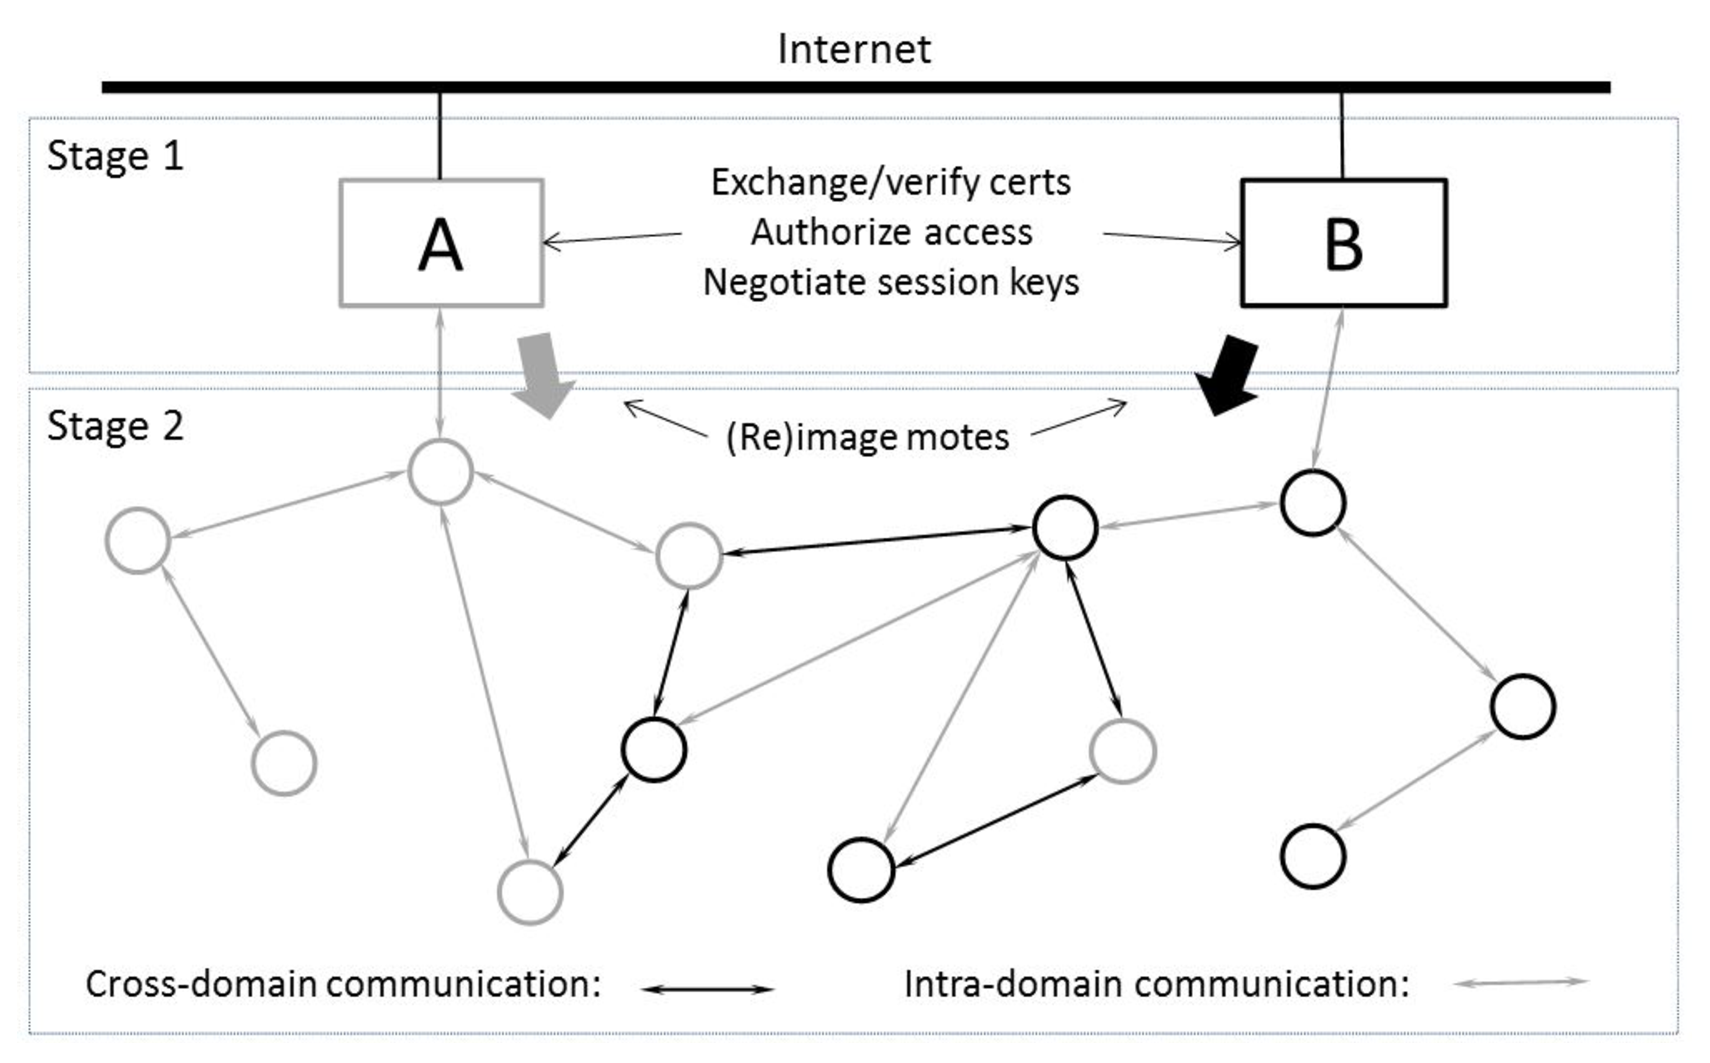
\includegraphics[scale=.40]{Figures/spartanrpc.eps}
  \end{center}
\end{fpfig*}

In some applications it may be desirable for the networks to share certain information while
keeping other information private. As one example, $A$ and $B$ may agree to use each other's
nodes for accurate time synchronization to their mutual best interest without wanting to share
any other functionality. Alternatively, perhaps the networks are willing to carry data from
foreign isolated nodes thus increasing each other's connectivity and enhancing their useful
lifetimes, all without being able to access each other's primary functions.

In other scenarios one of the networks, say $B$, may be reduced to a single mobile node that
wanders into the field of an established network $A$. In that case $B$ may wish to query $A$ or
otherwise interact with it, yet $A$ and $B$ may have no prior association.
\autoref{section-field-example} describes a specific scenario of this type used during the
evaluation of the work presented here.

Trust management systems provide exactly the kind of flexible, policy-driven authorization
control needed to address these situations. The ability to define access policy for unknown
principals, the hallmark of trust management, is particularly important in the case of mobile
embedded systems where encountering new principals is routine.

SpartanRPC addresses this problem directly by providing a way for the embedded devices
themselves to execute trust management logic. In that case no additional supporting
infrastructure is needed but the nodes are required to do extensive computations.

Scalaness, as a staged programming system, requires support beyond the nodes where the first
stage program can execute. This additional support is shown on top of
\autoref{figure-motivation} where Scalaness programs execute on the base stations of $A$ and $B$
to compute node programs for deployment that are specialized with appropriate session keys. The
Scalaness programs can communicate over the Internet to share credentials or other security
tokens as required.

\section{Security Model}

%%%%%
% Security model. Where to put it?
%%%%%

Although many security properties may be of interest to embedded systems applications, only one
is the focus of this work: \emph{a system is said to be secure if only authorized users of a
  resource can access it}. In this context a \newterm{resource} could be a physical device on a
node, e.g., a sensor or an actuator, or it could be a software component providing, e.g., a
computation, communication, or storage service. Each resource is presumed to have an
\newterm{authorizer} who controls access to that resource. A user is authorized for a resource
only if the authorizer's access policy for that resources grants that access.

Other security properties are not directly supported by this work. Notably, neither SpartanRPC
nor Scalaness address the issue of node tampering or denial of service attacks. Issues of data
confidentiality and message replay attacks are also outside the immediate scope of this work.

However, SpartanRPC and Scalaness do not interfere with the addition of other security services
to an application. For example an application specific protocol that adds nonces to messages
could be layered on top of either system to protect against replay attacks. Scalaness, in
particular, could be used to support such an approach by letting a first stage program compose
and specialize such a mechanism.

As usual it is assumed that the cryptographic primitives used by both systems are secure in the
sense that it is computationally infeasible for any attacker of interest to defeat the
cryptographic protections directly.

%%%%%
% End of security model.
%%%%%

\section{Related Work}

% From the Trust Management paper.

The first trust management systems were inspired by early foundational work in authentication
logics such as BAN \cite{Burrows:LA} and authorization logics such as ABLP \cite{Abadi:CACDS}.
However, the concept of trust management as an independent area of study was first introduced
with PolicyMaker \cite{Blaze:DTM,Blaze:CCPTMS}. PolicyMaker policies are implemented as
arbitrary programs in a suitable ``safe'' programming language. This gives the system great
flexibility but also introduces intractability.

KeyNote \cite{RFC-2704} is a direct descendant of PolicyMaker. KeyNote restricts PolicyMaker by
specifying a limited language for creating policies. However, a full analysis of KeyNote's
policy language \cite{Li:DCFTML} shows that certain authorization problems nevertheless remain
undecidable. KeyNote has been used to enforce IPsec security requirements
\cite{Blaze:TMIPS,Blaze:EKTMS}.

SDSI/SPKI \cite{Rivest:SDSI-11,RFC-2693} provides a relatively simple, yet expressively
interesting trust management language that is a precursor to the $RT_0$ system used here. The
semantics of SDSI/SPKI have been analyzed by several authors
\cite{Abadi:OSLLNS,Halpern:LSSLLNS,Howell:FSS,Li:LNSS,Clarke:CCDSS} making it one of the best
studied trust management systems. SDSI/SPKI has been used to provide security in component based
programming language design \cite{Liu:CSI}.

QCM \cite{Gunter:DALSI,Gunter:GCR} and its successor SD3 \cite{Jim:STMSCE,Jim:DDQE} cast
distributed authorization as a kind of distributed database problem. As a result, these systems
are able to leverage well-studied database techniques and abstractions. These systems reveal a
deep and interesting connection between authorization logics and database theory that inspired
later work with database query languages such as \datalog\ and \datalogc\ \cite{Li:DCFTML}.

Other notable examples of trust management systems include Cassandra \cite{Becker:CFTMAEHR}, a
system that has been studied in the context of the United Kingdom's proposed nationwide
electronic health records system, and the Extensible Access Control Markup Language (XACML)
\cite{OASIS:XACMLTC} and the Security Assertion Markup Language (SAML) \cite{OASIS:SSTC},
defining XML policy and assertion languages that make use of many trust management concepts.

% From the TISSEC paper.

Extending sensor network software platforms with support for secure interactions between domains
has been studied in previous research on SSL for sensor networks \cite{10.1109/WAINA.2009.47}.
However, this work was focused on extending the Internet to sensor networks (aka ``IP for
WSNs''), whereas SpartanRPC is a more general system for enhancing secure communications
\emph{within} a sensor network. Research on sensor network security has also addressed secure
routing \cite{senroute-ahnj03}, link layer security \cite{karlog-tinysec-2004}, cryptography
\cite{bertoni-2006}, key distribution \cite{camtepe-bulent-05}, and hardware issues
\cite{perrig-2004}. In contrast to these low-level systems, SpartanRPC provides language-level
abstractions for secure RPC services. Perhaps even more closely related is a system for
establishing fine-grained, ``node-level'' policies in sensor networks
\cite{Claycomb:2011:NNL:1889383.1889450}. However, this work is more focused on group-based key
negotiation and distribution, and while it does offer a policy language, it is rooted in
implementation details and not as a separable specification. Also, that work does not provide a
language API for integrating their system into secure applications as does SpartanRPC.

Previous related work also illustrates interest in and useful applications of RPC in embedded
networks. For example, the Marionette system uses network layer RPC for remote (PC-based)
analysis and debugging of sensor networks \cite{whitehouse-marionette-2006}. The Fleck operating
system provides a small pre-defined set of RPC services for sensor network applications, while
the trustedFleck system extends this with a form a secure RPC
\cite{hu-secfleck-2009,Hu:2010:TTW:1806895.1806900}. S-RPC provides an RPC facility for sensor
networks that allows remote services to be added to the system dynamically \cite{5766863}.
SpartanRPC differs from these systems in that it extends the nesC programming language (unlike
trustedFleck) to allow programmer definition of secure RPC services (unlike S-RPC) that can be
accessed by nodes within the network itself (unlike Marionette). SpartanRPC is similar to, and
inspired by, TinyRPC \cite{may-tinyrpc-2007}. TinyRPC, however, does not provide security and
has different semantics that are not as expressive as SpartanRPC's approach.

Teeny\textsc{lime} allows application programs to access an abstract ``tuple space'' that is the
union of tuple spaces on the local node and the immediately neighboring nodes
\cite{Costa:2007:PWS:1516124.1516153}. This provides an alternative to RPC for uniformly
accessing remote and local data. However, interaction with the middleware is by way of a
dedicated API; there is no attempt to provide a true RPC mechanism. Also Teeny\textsc{lime} does
not address issues of access control.

Secure Middleware for Embedded Peer to Peer systems (SMEPP) is a general framework for creating
security sensitive applications from a distributed network of embedded peers
\cite{Brogi:2008:SME:1363370.1363548}. SMEPP Light \cite{Vairo:2008:SMW:1594978.1595054} is a
reduced version of SMEPP to address the resource constraints of wireless sensor networks. SMEPP
Light provides a publish/subscribe communication model using directed diffusion
\cite{intanagonwiwat-2003} to distribute ``events'' to all subscribers and symmetric key
cryptography to provide confidentiality and data integrity within a group of nodes. However,
SMEPP Light is not integrated into a programming language and does not provide a remote
procedure call mechanism. Furthermore, SMEPP Light only supports a simple model of access
control based on group membership.

High level macro\-programming languages such as Kairos \cite{springerlink:10.1007/1150259312},
and Regiment \cite{Newton:2007:RMS:1236360.1236422} provide a way to program the entire network
as a single entity. These systems attempt to hide not only the inter-node communication from the
programmer, but also the entire node level programs. SpartanRPC operates at a much lower level
making it potentially more flexible and also, unlike these macro\-programming systems,
SpartanRPC addresses access control issues in networks containing multiple security domains.

Whole network programming of wireless sensor networks has also been investigated using mobile
agents in systems such as Agilla \cite{Fok:2009:AMA:1552297.1552299} and Wiseman
\cite{Gonzalez-Valenzuela:2010:PMW:1891545.1891566}. However, like the macro\-programming
systems mentioned previously, neither of these systems address issues related to access control
in the presence of multiple security domains.

% From the GPCE paper

The potential of applying staged metaprogramming techniques to sensor networks was explored in
the functional sensor language Flask \cite{Mainland-Flask-2008}. Flask allows functional
reactive programming (FRP)-based stream combinators to be pre-computed before network
deployment, but it is possible to generate ill-typed Flask object code since cross-stage static
type checking is not performed. Hume \cite{Hume} is a domain specific language for real-time
embedded device programming. It includes a metaprogramming layer but that layer is more like
nesC's configuration files in that there is a very restricted syntax for a few special
metaprogramming operations including component wiring, macros, and code templating.

MetaML \cite{Taha-MetaML,DBLP:conf/icess/Taha04} and MetaHaskell \cite{mainland12} are
foundations the work described here builds on. MetaHaskell does support heterogeneous language
staging where the lower stage language is defined by a plug-in and several instantiations have
been defined including one for a low-level C-like language. Like this dissertation's approach,
they guarantee type safety of all lower-stage code produced. They use a more traditional
metaprogramming model, however, not the process-separated model needed for embedded systems
metaprogramming and they do not address the issues of metaprogramming module composition and
type specialization. In contrast, Scalaness follows the foundational work on Framed ML (\fml)
\cite{FramedML}; \autoref{section-framedml} discusses how it serves as the theoretical
underpinning of the Scalaness system.

Lightweight Modular Staging \cite{Rompf-LMS} describes a method of expressing staged
computations using a Scala host framework without any compiler modifications. The approach
allows cross-stage type safety but does not support dynamic type construction, a method by which
second stage types can be manipulated as first stage values. This feature provided by Scalaness
is important for optimizing the layout of data structures by tuning the types used for their
members.

Actor based sensor metaprogramming has been studied in \cite{cheong07}; this work also focuses
on high level dynamic reprogrammability but is untyped. More broadly, metaprogramming is known
to be useful for increasing the efficiency of systems applications. One example is Tempo
\cite{289140}, a system that integrates partial evaluation and type specialization for
increasing efficiency of systems applications. Ur \cite{UrPLDI10} allows for type safe
metaprogramming for web applications.

The units of staged code composition in nesT are \emph{modules}. Countless different module
systems exist, but they are primarily designed to achieve separate compilation and sound linking
\cite{Cardelli-1997}.The different design goals of nesT lead to different design choices in nesT
modules. For example, data crossing nesT module boundaries needs to conform to the property of
process separation, a non-issue in standard module system designs. In addition, nesT modules
allow values/types across the boundary of modules to be flexibly constructed, including dynamic
construction of types. Module systems such as ML modules \cite{macqueen84} and Units
\cite{flatt98units} allow types to be imported/exported as Scalaness supports. However, there
are several features of ML modules including type hiding that Scalaness does not aim to support.

NesT modules are more expressive in their support of first class modules as values and the
possibility of dynamic construction of ``type exports.'' That said, first class modules are not
new \cite{99620,ancona01calculus}. The novelty of nesT arises in its application to program
staging and the incorporation of dynamic type construction.

The type parametricity of System F and F$_\le$ \cite{Cardelli-1985}, and the practical type
systems it inspired such as Java's generics, do not treat types as first class values. C++
templates support types as meta values in template expansion, but type safety of generated code
is not guaranteed without full template expansion. Concepts \cite{gregor06:_concepts} improves
on this, but types are still not first class values.

The main contributions of this work include a demonstration, for the first time, of the
feasibility of using trust management in resource constrained embedded systems. The SpartanRPC
language, together with its implementation in \Sprocket, provide for a direct approach to
solving the trust management problem. The staged Scalaness/nesT system treats the trust
management problem as simply one possible application of many. Scalaness offers a unique
combination of staging with process separation, cross-stage type safety, and dynamic type
construction that make it a powerful tool for creating flexible and efficient embedded
applications.

\section{Dissertation Organization}

The rest of this dissertation is organized as follows. Trust management systems are described,
in general, in \autoref{chapter-trust-management}, outlining the different features provided by
common trust management systems and motivating their use. Special focus is given to the \RT\
family of trust management systems used in this work. The design of SpartanRPC is described, as
well as the details of its implementation, in \autoref{chapter-spartanrpc-sprocket}. Of
particular note is the description of the added support for $RT_0$ trust management to a general
RPC mechanism. Scalaness and nesT are introduced in more detail in
\autoref{chapter-dscalaness-dnest}, and then the syntax and semantics of both languages are
described, using simplified ``distilled'' versions of those languages called
\newterm{DScalaness} and \newterm{DnesT}. The implementation of the practical Scalaness/nesT
system is described in \autoref{chapter-scalaness-nest}, relating the features of the
implementation to the earlier foundational presentation. An evaluation of both systems is
provided in \autoref{chapter-evaluation} using simple test programs in the context of a
realistic field example. The conclusion is documented in \autoref{chapter-conclusion}. Finally,
in \autoref{chapter-sample} the full source code of a simple Scalaness/nesT sample is
demonstrated, with commentary.

%%% Local Variables: 
%%% mode: LaTeX
%%% TeX-master: "main"
%%% End: 
